\chapter{Anticliques in Graphs of Polytopes}
\label{chap:Anticliques}

Let \(G=(V, E)\) be a graph.  An \dfn{anticlique} is a subset \(A\) of \(V\) (of cardinality at least \(2\)) such that \(E\cap\binom A2=\mt\).  If \(\card A=k\), then \(A\) is said to be a \(k\)-anticlique.  A \(2\)-anticlique is simply a nonedge.

Recall that if \(G\) is the graph of a \(d\)-polytope \(P\) with \(n\) vertices, and \(\Gamma\in\galed(P)\) is a Gale diagram of \(P\), then \(\seta{{\ve v}_i,{\ve v}_j}\) is a nonedge of \(P\) if and only if there is some hyperplane \(H_{i,j}\sbset\R{n-d-1}\) containing \(\ve0\) such that \(H_{i,j}^{(+)}\cap\Gamma=\seta{\ol{\ve v}_i,\ol{\ve v}_j}\).  Such a hyperplane is called a \dfn{separating} hyperplane.  The normal vector to \(H_{i,j}\) which has positive inner product with \(\ol{\ve v}_i,\ol{\ve v}_j\) and norm \(1\) is denoted \(\ve x_{i,j}\).

If \(P\) is a \(d\)-polytope with \(d+k\) vertices, then Theorem \ref{Thm:ConnectivityOfGraph} in Section \ref{Sec:GraphsOfPolytopes} implies that each vertex of \(\gr P\) must have degree at least \(d\).  If a graph \(H\) with \(d+k\) vertices has a \((k+1)\)-anticlique, then each vertex in the anticlique has degree at most \(d-1\), and hence \(H\) is not \(d\)-realizable.  However, the graph \(\left(\brac{d+k},\binom{\brac{d+k}}2\setminus\binom{\brac k}2\right)\) is \(d\)-connected, and furthermore has a \(K_{d+1}\) minor (the induced subgraph on the vertex set \(\seta{k, k+1\dc k+d}\) is complete) and thus \emph{could} be the graph of a \(d\)-polytope.  It will be shown that this cannot happen.  More precisely for \(k\ge 2\), let
    \[
        f(d,k)=\max\setb{n}{\text{there is some \(d\)-polytope \(P\) with \(d+k\) vertices and an \(n\)-anticlique}}.
    \]
Then the goal is to show that \(f(d,k)<k\) for \(k>2\).

\section{An Upper Bound on \protect$f\protect$}
First note that \(f\) is weakly increasing in both arguments.

\begin{Theorem}\ph
    \begin{enumerate}
        \item   \(f(d,k)\le f(d+1,k)\)
        \item   \(f(d,k)\le f(d,k+1)\)
    \end{enumerate}
\end{Theorem}
\begin{proof}
    Let \(P\) be a \(d\)-polytope with \(d+k\) vertices, and an \(f(d,k)\)-anticlique.
        \begin{enumerate}
            \item   The \((d+1)\)-polytope \(\pyr(P)\) has \((d+k)+1=(d+1)+k\) vertices and an \(f(d,k)\)-anticlique.
            \item   Let \(F\) be any facet of \(P\).  The \(d\)-polytope \(K(P;F)\) (defined in section \ref{Subsec:Kleetopes}) has \(d+(k+1)\) vertices and an \(f(d,k)\)-anticlique.
        \end{enumerate}
\end{proof}



Recall that a standard Gale diagram is one in which each point is either on the unit sphere, or at the origin.  Further if a point in the Gale diagram is at the origin, then the polytope is a pyramid with apex the corresponding point.  Since the main question is concerned with sizes of anticliques, and the anticliques of a pyramid are exactly those of its base, nothing is lost or gained in the assumption that a polytope is not a pyramid.

\begin{Theorem}\label{Thm:TrivialitiesAnticliques}
    Let \(P\) be a \(d\)-polytope with vertex set \(\seta{\ve v_1,\ve v_2\dc\ve v_{n}}\);  \(A=\seta{i_1,i_2\dc i_k}\sbset\brac n\); \(\setb{\ve v_{i}}{i\in A}\) be an anticlique;  \(\Gamma\) be a standard Gale diagram of \(P\); and \(\seta{i,j}\sbset A\).  Then
        \begin{enumerate}
            \item   \(\ol{\ve v}_i\ne\ve 0\).
            \item   \(\ol{\ve v}_i\ne-\ol{\ve v}_j\).
        \end{enumerate}
    Furthermore if \(k\ge3\), then
        \begin{enumerate}[resume]
            \item\label{ThmPt:notequal}   if \(\ol{\ve v}_i=\ol{\ve v}_j\) , then \(i=j\).
        \end{enumerate}
\end{Theorem}
\begin{proof}\ph
    \begin{enumerate}
        \item   If \(\ol{\ve v}_i=\ve 0\), then \(\conv\seta{\ve v_i,\ve v_t}\) is a face of \(P\) for each \(t\in\brac n\setminus\{i\}\).  In particular, \(\conv\seta{\ve v_i,\ve v_j}\) is an edge of \(G(P)\).
        \item  If \(\ol{\ve v}_i=-\ol{\ve v}_j\),and \(H_{i,j}\) is a separating hyperplane for \(\ol{\ve v}_i,\ol{\ve v}_j\) with normal vector \(\ve x_{i,j}\), then
                \[
                    0<\ip{\ve x_{i,j}}{\ol{\ve v}_i}=-\ip{\ve x_{i,j}}{\ol{\ve v}_j}<0.
                \]
        \item  Let \(H_{a,b}\) be a separating hyperplane for \(\ol{\ve v}_a,\ol{\ve v}_b\) with normal \(\ve x_{a,b}\) for each pair \(a,b\in A\).  Suppose \(\ol{\ve v}_i=\ol{\ve v}_j\) with \(i\ne j\).  Then for \(r\in A\setminus\seta{i,j}\),
                \[
                    0   <\ip{\ve x_{j,r}}{\ol{\ve v}_j}
                        =\ip{\ve x_{j,r}}{\ol{\ve v}_i}
                        \le 0.
                \]
            Hence \(i=j\).\qedhere
    \end{enumerate}
\end{proof}
\begin{Theorem}
    \(f(d,2)=2\)
\end{Theorem}
\begin{proof}
    If \(P\) is a \(d\)-polytope with \(d+2\) vertices, then \(P\) has a \(1\)-dimensional Gale diagram.  Since a nonedge requires that there be a separating hyperplane, and in this case there is only one possible hyperplane (namely the origin), each vertex can have at most one nonneighbor.  This implies that \(f(d,2)\le2\).  The polytope \(\pyr_{d-2}(\xp2)\) is \(d\)-dimensional with \(d+2\) vertices and a \(2\)-anticlique.  Thus \(f(d,2)=2\).
\end{proof}
\begin{Theorem}
    \(f(d,3)<3\)
\end{Theorem}
\begin{proof}
    Let \(P\) be a \(d\)-polytope with \(d+3\) vertices, and let \(\Gamma\) be  a standard Gale diagram of \(P\).  Suppose that \(P\) has a \(3\)-anticlique \(\seta{\ve v_1,\ve v_2,\ve v_3}\), and let \(\ve v_4\) be any other vertex of \(P\).  Note that since \(\Gamma\sbset\Sp1\) (assuming again that \(P\) is not  a pyramid), by writing each \(\ol{\ve v}_i\in\Gamma\) in polar coordinates only the angle \(\varphi_i\in[0,2\pi)\) is necessary to specify \(\ol{\ve v}_i\).  By Theorem \ref{Thm:TrivialitiesAnticliques} part \ref{ThmPt:notequal}, none of \(\varphi_1,\varphi_2,\varphi_3\) are equal, so assume \(\varphi_1<\varphi_2<\varphi_3\).  Further, if \(\varphi_1>0\), then rotating each point in \(\Gamma\) clockwise by an angle of \(\varphi_1\) produces a consubstantial standard Gale diagram, so assume
        \[
            0=\varphi_1<\varphi_2<\varphi_3<2\pi.
        \]

        \begin{center}
            \begin{figure}[h!bt]
                \includegraphics[page=23, width=.3\textwidth]{pictures.pdf}
            \end{figure}
        \end{center}

    Since \(\ve v_1\ve v_2\) is not an edge of \(P\), there is some hyperplane \(H_3\) through the origin such that \(H_3^{(+)}\cap\Gamma=\seta{\ol{\ve v}_1,\ol{\ve v}_2}\).  Therefore, \(\varphi_4\notin[0,\varphi_2]\).  Similarly, \(\varphi_4\notin[\varphi_2,\varphi_3]\), and \(\varphi_4\notin[\varphi_3,2\pi)\).  Since \(\Gamma\) is a standard Gale diagram, this means that \(\ol{\ve v}_4=\ve0\).  But this contradicts the assumption that \(P\) is not a pyramid.
\end{proof}


\begin{Lemma}\label{Lem:LocalCone}
    If
        \begin{itemize}
            \item   \(P\) is a \(d\)-polytope with vertex set \(V\cup Y\) of cardinality \(d+k\),
            \item   \(\card V=d\) and \(\card Y=k\),
            \item   \(Y\) is an anticlique of \(\gr P\), and
            \item   \(\ve v\in V\), then
        \end{itemize}
    \(\ve v\ve y\) is an edge of \(\gr P\) for each \(y\in Y\).
\end{Lemma}
\begin{proof}
    Let \(\ve v\in V\), \(\ve y\in Y\).  Since \(P\) is a \(d\)-polytope, it is \(d\)-connected, therefore each vertex of \(G(P)\) is adjacent to at least \(d\) other vertices.  But since \(Y\) is an anticlique, \(\ve y\) is adjacent to at most \(d\) other vertices. Hence \(\ve y\) is adjacent to exactly \(d\) other vertices, and since none of these other vertices is in \(Y\), \(\ve v\ve y\) is an edge of \(G(P)\).
\end{proof}

    The following is a general fact about polytopes.  A proof is included for completeness, but
\begin{Lemma}\label{Lem:LocallySimple}
    Let \(P\) be a \(d\)-polytope, \(\ve y\in\vrt P\) with \(\deg\ve y=d\), and \(V=N(\ve y)=\seta{\ve v_1,\ve v_2\dc\ve v_d}\).  Then for each subset \(X\) of \(V\) with cardinality \(d-1\) there is a unique facet \(F\) of \(P\) with \(X\sbset\vrt F\).
\end{Lemma}
\begin{proof}
    Each vertex of \(P\) lies in at least \(d\) facets since \(P\) is a \(d\)-polytope.  Let \(F\) be a facet containing \(\ve y\).  Since \(F\) is a \((d-1)\)-polytope, each vertex of \(G(F)\) has degree at least \(d-1\).  Thus \(\ve y\) must have either \(d-1\) or \(d\) neighbors in \(F\).  If \(\ve y\) had each of its \(d\) neighbors in \(F\), then \(\ve y\) would only lie in one facet.  Thus each facet in which \(\ve y\) lies contains exactly \(d-1\) neighbors of \(\ve y\).  Further, each element of \(\binom V{d-1}\) determines a unique facet of \(P\) since \(\ve y\) lies in at least \(d\) facets.
\end{proof}

Notice that this argument also shows that the set \(V\) above is affinely independent, and that \(V\) is not contained in any proper face of \(P\).

\begin{Theorem}\label{Thm:Anticliques}
    If \(k>2\), then \(f(d,k)<k\).
\end{Theorem}
\begin{proof}
    Proceed by induction on \(d\).  For the base case: the graph of a \(2\)-polytope with \(n\) vertices is a cycle of length \(n\), so a maximal anticlique can be obtained by taking every other vertex. Therefore \(f(2,k)=1+\floor{k/2}<k\).  Thus, suppose  for some \(d\) that \(f(d-1,k)<k\) for all \(k>2\).  The proof of the contrapositive will be shown, that is, if \(f(d,k)=k\), then \(k=2\).

    Let \(P\) be a \(d\)-polytope with \(d+k\) vertices and, without loss of generality, suppose that \(P\) is not a pyramid.  Suppose further, that \(P\) has a \(k\)-anticlique \(Y=\seta{\ve y_1,\ve y_2\dc\ve y_k}\).  Write \(\vrt(P)=\seta{\ve v_1,\ve v_2\dc\ve v_d}\cup Y\), let \(V=\seta{\ve v_1,\ve v_2\dc\ve v_d}\), and \(V_i=V\setminus\seta{\ve v_i}\) for \(i\in\brac d\).  Fix some \(i\in\brac d\), and for each \(j\in\brac k\), let \(F_{i,j}\) be the facet of \(P\) which contains \(V_i\cup\seta{\ve y_j}\) (Lemmata \ref{Lem:LocalCone} and \ref{Lem:LocallySimple}), and \(G_i\) be the smallest face of \(P\) which contains \(V_i\).

    Notice that \(G_i\sbset F_{i,j}\) for each \(j\in\brac k\), and that \(G_i\) is either a facet or a ridge since \(V\) is an affinely independent set.

        \begin{enumerate}
            \item   (\(G_i\) is a facet.)  In this case, for each \(j\in\brac k\), \(G_i=F_{i,j}=\conv(Y\cup V_i)\).  Thus \(P\) is a pyramid over \(G_i\) with apex \(\ve v_i\).  This is a contradiction.
            \item   (\(G_i\) is a ridge.)  Let \(F_1,F_2\) be the facets containing \(G_i\).  In this case, \(Y\) can be partitioned into two nonempty sets
                    \begin{align*}
                        Y_1 &=  \seta{\ve y_{a_1},\ve y_{a_2}\dc\ve y_{a_r}}&
                        Y_2 &=  \seta{\ve y_{b_1},\ve y_{b_2}\dc\ve y_{b_s}}&
                    \end{align*}
                such that
                    \begin{align*}
                        Y_1 &\sbset F_{i,a_1}   =   F_1&
                        Y_2 &\sbset F_{i,b_1}   =   F_2.&
                    \end{align*}

                If \(\card{Y_1}=2\), then \(F_1\) is a \((d-1)\)-polytope with \((d-1)+2\) vertices and \(G_i\) is a facet of \(F_1\).  Thus a Gale diagram of \(F_1\) is one dimensional with \(d+1\) vertices, and both \(\ol{\ve y}_{a_1}\) and \(\ol{\ve y}_{a_2}\) are on the same side of the origin.  However, \(\ve 0\in\relint\conv{\left(\ol{\vrt(F_1)\setminus Y_1}\right)}\).  Similarly, \(\card{Y_2}\ne2\).

                If \(\card{Y_1}\ge 3\), then \(F_{i,a_1}\) is a \((d-1)\)-polytope with \((d-1)+\card{Y_1}\) vertices, and a \(\card{Y_1}\)-anticlique, that is, \(f(d-1,\card{Y_1})\ge\card{Y_1}\).  This contradicts the inductive hypothesis.

                Hence \(\card{Y_1}=\card{Y_2}=1\), whence \(P\) is a \(d\)-polytope with \(d+2\) vertices and a \(2\)-anticlique.  Thence \(k=2\).
        \end{enumerate}
\end{proof}

\section{A Lower Bound on \protect$f\protect$}

\begin{Lemma}
    If
        \begin{itemize}
            \item   \(P\) is a \(d\)-polytope with \(d+k\) vertices,
            \item   \(\ve v\) is a vertex of \(P\) such that each facet containing \(\ve v\) is a simplex, and
            \item   \(\ve v\) is contained in a \(q\)-anticlique of \(P\), then
        \end{itemize}
    \(f(d,k+i)\ge q+i-1\) for \(i\in\brac d\).
\end{Lemma}
    For example, such a vertex exists when \(P\) is a simplex (in which case each vertex has this property) or if \(P\) is of the form \(P=K(P';F)\) where \(F\) is a facet of \(P'\) which is a simplex, so the Lemma is not vacuous.
\begin{proof}
    Let \(F_1,F_2\dc F_d\) be facets of \(P\) containing \(\ve v\), and set
        \begin{align*}
            P_0(\ve v)
                    &=P\\
            P_i(\ve v)
                    &=K(P;F_1,F_2\dc F_i)\\
            \seta{\ve v_i}
                    &=\vrt(P_i(\ve v))\setminus\vrt(P_{i-1}(\ve v)).
        \end{align*}
    Further, let \(A'\) be a \(q\)-anticlique of \(P\) which contains \(\ve v\), and set \(A=A'\setminus\seta{\ve v}\).

    For a fixed \(i\in\brac d\), the inclusion \(N(\ve v_i)\sbset N(\ve v)\cup\seta{\ve v}\) in \(\gr{P_i(\ve v)}\) implies that  \(A\cup\seta{\ve v_1,\ve v_2\dc\ve v_i}\) is a \((q-i-1)\)-anticlique in \(\gr{P_i(\ve v)}\).
\end{proof}

\begin{Theorem}\label{Thm:Bounds}
    If \(k,d>2\), then \(\ds k-1-\floor{\frac{k-3}d}\le f(d,k)\le k-1\).
\end{Theorem}
\begin{proof}
    Fix \(d>2\) and set \(t=\floor{(k-3)/d}\) and let \(Q_0=K(\simp d;F)\) for some facet \(F\) of \(\simp d\).  Let \(\ve v_0\) be a vertex of \(Q_0\) and \(F_{0,1},F_{0,2}\dc F_{0,d}\) be the facets of \(Q_0\) which contain \(\ve v_0\).  Then for \(k\in\brac{d}\), the polytope \(K(Q_0;F_{0,1},F_{0,2}\dc F_{0,k})\) is a \(d\)-polytope with \(d+2+k\) vertices and a \((k+1)\)-anticlique.  Now, inductively define, for \(n\in\N\setminus\seta0\), the polytope
        \[
            Q_n
                =
                    K(Q_{n-1};F_{n-1,1},F_{n-1,2}\dc F_{n-1,d})
        \]
    where \(\seta{F_{n-1,1},F_{n-1,2}\dc F_{n-1,d}}\) is the set of facets that contain some fixed vertex in a maximal anticlique of \(Q_{n-1}\).

    Finally, for \(k\in\brac{d}\) the polytope \(K(Q_n;F_{n,1},F_{n,2}\dc F_{n,k})\) is a \(d\)-polytope with \(d+(nd+2+k)\) vertices and an anticlique of cardinality \(nd+2+k-n-1\).
\end{proof}

Notice that if \(\floor{(k-3)/d}=0\) (that is, \(k\le d+2\)), then the upper and lower bounds on \(f\) agree.

\section{The Value of \protect$f\protect$ in Dimension \protect$3\protect$}

If \(d=3\), then Theorem \ref{Thm:Bounds} says that \( k-1-\floor{(k-3)/3}\le f(3,k)\le k-1\).  In this case, the lower bound can be rewritten as \(\ds k-1-\floor{(k-3)/3}=\ceil{2k/3}\).

    \subsection{Euler's Theorem}
        Euler's Theorem states that the \(f\)-vector of a \(d\)-polytope lies on a certain hyperplane in \(\R{d}\).  For a proof, see \cite{GrunBook}, \cite{McMullenBook}, or \cite{ZieglerBook}.  All that will be needed is the \(d=3\) case:
            \begin{Theorem}[Euler]
                If \(P\) is a \(3\)-polytope, then \(f_0(P)-f_1(P)+f_2(P)=2\).
            \end{Theorem}
        Euler's Theorem can be proven for planar graphs in general; in this case \(f_2\) counts the number of regions into which the graph divides the plane.

        Since each region of a planar graph is bounded by at least \(3\) edges, and each edge lies on at most \(2\) facets, \(3R\le2\card{E(G)}\) where \(R\) is the number of regions into which the graph divides the plane.  If \(G\) is the graph of a polytope \(P\), then \(R=f_2(P)\).  If the number of edges bounding a region is at least \(4\), then this inequality becomes \(4R\le2\card{E(G)}\), i.e.{}, \(2R\le\card{E(G)}\).  Combining this with Euler's Theorem yields \(\card{E(G)}\le3\card{V(G)}-6\) for a general planar graph, and \(\card{E(G)}\le2\card{V(G)}-4\) for a planar graph with no \(3\)-cycles.  In particular, if \(G\) is bipartite, then it has no \(3\)-cycles.

    \subsection{Bipartite Graphs Induced by Anticliques}

    If \(P\) is a \(3\)-polytope and \(A\) is an anticlique of \(G=\gr P\), then \(A\) induces a bipartite graph \(G_A\) whose vertex set is that of \(G\), and whose edge set is the set of edges in \(G\) which contain a vertex of the anticlique \(A\).  That is:
        \begin{align*}
            V(G_A)
                &=  V(G)\\
            E(G_A)
                &=  \setb{ax}{a\in A}\cap E(G).
        \end{align*}
    Note that \(G_A\) is planar since \(G\) is planar, and \(G_A\) is a subgraph of \(G\).

    \begin{Theorem}
        \(f(3,k)=\ceil{2k/3}\)
    \end{Theorem}
    \begin{proof}
        Suppose that \(P\) is a \(3\)-polytope with \(3+k\) vertices and a \((\ceil{2k/3}+1)\)-anticlique \(A\).  Let \(G=\gr P\) and \(a\in A\).  Since each edge of \(G\) on which \(a\) lies is also an edge of \(G_A\), and \(a\) lies on at least \(3\) edges of \(G\), it follows that
            \begin{align*}
                \card{E(G_A)}
                    &\ge
                        3(\ceil{2k/3}+1)
                    \ge
                        3(2k/3+1)
                    =
                        2k+3
            \end{align*}
        On the other hand, \(G_A\) is a bipartite planar graph with \(3+k\) vertices.  It therefore has at most \(2(3+k)-4=2k+2\) edges.
    \end{proof}




    \begin{table}[h]
    \begin{tabular}{c|ccccccccccccccc}
       \multicolumn{1}{l|}{\backslashbox[0pt][]{d\kern-5em}{\kern-.5em k}}   & \(\vphantom{\ds\sum_a^b}\)2 & 3 & 4 & 5 & 6        & 7        & 8        & 9        & 10       & 11       & 12        & 13        & 14        & 15        & 16        \\\hline
        2 & 2 & 2 & 3 & 3 & 4 & 4 & 5 & 5 & 6 & 6 & 7 & 7 & 8  & 8   & 9 \\
        3 & 2 & 2 & 3 & 4 & 4 & 5 & 6 & 6 & 7 & 8 & 8 & 9 & 10 & 10 & 11 \\
        4 & 2 & 2 & 3 & 4 & 5 & \(\mbf5\) & \(\mbf6\) & \(\mbf7\) & \(\mbf8\) & \(\mbf8\) & \(\mbf9\)  & \(\mbf{10}\) & \(\mbf{11}\) & \(\mbf{11}\) & \(\mbf{12}\) \\
        5 & 2 & 2 & 3 & 4 & 5 & 6 & \(\mbf6\) & \(\mbf7\) & \(\mbf8\) & \(\mbf9\) & \(\mbf{10}\) & \(\mbf{10}\) & \(\mbf{11}\) & \(\mbf{12}\) & \(\mbf{13}\) \\
        6 & 2 & 2 & 3 & 4 & 5 & 6 & 7 & \(\mbf7\) & \(\mbf8\) & \(\mbf9\) & \(\mbf{10}\) & \(\mbf{11}\) & \(\mbf{12}\) & \(\mbf{12}\) & \(\mbf{13}\) \\
        7 & 2 & 2 & 3 & 4 & 5 & 6 & 7 & 8 & \(\mbf8\) & \(\mbf9\) & \(\mbf{10}\) & \(\mbf{11}\) & \(\mbf{12}\) & \(\mbf{13}\) & \(\mbf{14}\) \\
        8 & 2 & 2 & 3 & 4 & 5 & 6 & 7 & 8 & 9 & \(\mbf9\) & \(\mbf{10}\) & \(\mbf{11}\) & \(\mbf{12}\) & \(\mbf{13}\) & \(\mbf{14}\) \\
        9 & 2 & 2 & 3 & 4 & 5 & 6 & 7 & 8 & 9 & 10 & \(\mbf{10}\) & \(\mbf{11}\) & \(\mbf{12}\) & \(\mbf{13}\) & \(\mbf{14}\)\\
        10& 2 & 2 & 3 & 4 & 5 & 6 & 7 & 8 & 9 & 10 & 11 & \(\mbf{11}\) & \(\mbf{12}\) & \(\mbf{13}\) & \(\mbf{14}\)\\
        11& 2 & 2 & 3 & 4 & 5 & 6 & 7 & 8 & 9 & 10 & 11 & 12 & \(\mbf{12}\) & \(\mbf{13}\) & \(\mbf{14}\)
    \end{tabular}\caption{Values of \protect$f(d,k)\protect$.  Numbers in bold are lower bounds.}
    \end{table}





    \begin{comment}
    \begin{figure}[hbt]
        \centering
            \includegraphics[width=.7\textwidth, page=14]{pictures.pdf}
        \caption{The polytope $\xp 3$ and a Gale transformation of its vertices.\label{Fig:xp3Gale}}
    \end{figure}
    \end{comment}
\begin{comment}
Note that it is possible to have an anticlique of size \(2\) for which (what the hell was I trying to say here?)

    If \(P\) is a \(d\)-polytope, and \(G\in\galed(P)\) is a Gale diagram of \(P\), then it is a simple matter to determine \(\gr P\), the graph of \(P\), from \(G\).  A \dfn{coedge} of a polytope \(P\) is a coface which corresponds to an edge of \(P\).  By Theorem \ref{Thm:CofaceIFF}, the set \(X=\seta{\ve x_1,\ve x_2}\sbset\vrt P\) (\(\ve x_1\ne\ve x_2\))  is a coedge if and only if \(\ol{ V\setminus X}\) either captures the origin, or is empty.  This condition can only fail if there is some hyperplane \(H\) containing \(\ve 0\) such that \(\ol X= G\cap H^{(+)}\).  Thus the nonedges of the graph of a polytope can be determined from a Gale diagram easily.
\end{comment}
